\section{Introduzione}

Lo scopo di questa esperienza di laboratorio è quello di montare di un impianto da vuoto che risulti in
grado di raggiungere pressioni dell'ordine di $10^{-3}$ \si{\pascal}. Inoltre l'esperienza serve anche a
prendere dimestichezza con le varie componenti che costituiscono l'impianto da vuoto.
Infine l'ultimo obbiettivo, ad impianto funzionante, è quello di tarare un vacuometro Pirani.

\section{Materiale utilizzato}

Il materiale messo a nostra disposizione è il seguente:

\begin{itemize}
	\item{una camera con un volume di $5930 \pm 10$ \si{\centi\metre}$^3$;}
	\item{una pompa rotativa con pressione di vuoto limite dell'ordine di qualche Pascal;}
	\item{una pompa turbomolecolare-molecular drag con relativa elettronica;}
	\item{cravatte e O-ring in Viton di varie dimensioni;}
	\item{tubi con flange quanto basta;}
	\item{2 valvole a membrana, 1 valvola a perdita calibrata, 1 valvola gate;}
	\item{2 vacuometri Pirani, 1 vacuometro a ionizzazione a catodo caldo e 1 vacuometo a ionizzazione a catodo freddo;}
	\item{cavi e lettore AGC per i quattro sensori sopracitati;}
\end{itemize}

\section{Esecuzione dell'esperienza}

\subsubsection{Montaggio dell'impianto da vuoto}

Per quanto riguarda il montaggio dell'impianto da vuoto abbiamo utilizzato il materiale sopraelencato,
prestando attenzione che fossero rispettate le richieste dei tecnici di laboratorio,
ovvero che l'impianto soddisfacesse i seguenti requisiti:

\begin{itemize}
	\item{si doveva poter isolare la pompa turbomolecolare dal resto dell'impanto. In pratica abbiamo realizzato un bypass
    dotato di valvola che collegava la pompa rotativa direttamente con la camera. In questo modo è possibili portare la camera a
    temperatura atmosferica senza spegnere la pompa turbomolecolare (che tra l'altro ci mette parecchi minuti a fermarsi);}
	\item{si doveva avere la possibilità di riportare la camera da vuoto alla pressione atmosferica senza spegnere
    la pompa turbomolecolare, che lavora correttamente in regime molecolare, ossia a pressioni inferiori a qualche Pascal;}
\end{itemize}

Uno schema dell'impianto è riportato in figura \ref{fig:schema}.

\subsubsection{Taratura dei vacuometri Pirani}

Per tarare il vacuometro Pirani, che misurava la pressione in camera,
abbiamo portato la pressione oltre il limite inferiore
della sensibilità dello strumento, specificato nel manuale. Abbiamo quindi impostato il
voltaggio in uscita al valore di 2 Volt. Dopo aver isolato la pompa turbomolecolare dal resto
dell'impianto, abbiamo riportato la pressione della camera alla pressione atmosferica e
imposatato il valore di output del sensore a 10 Volt. Abbiamo quindi riportato la pressione in
camera a passa pressione per controllare che il voltaggio al limite inferiore fosse ancora 2 Volt.

\subsubsection{Qualche dato}

La pressione da noi raggiunta, come misurata con il vacuometro a catodo caldo, è di circa:

\begin{equation}
    P = 6.45 \text{(controllare per piacere)} \cdot 10^{-4} \; \si{\pascal}
\end{equation}

\begin{figure}[b!]
    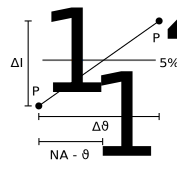
\includegraphics[width=14.5cm]{drawing.pdf}
    \caption{Schema dell'impianto da noi realizzato.}
    \label{fig:schema}
\end{figure}
